
Para el estudio del m\'etodo de generaci\'on de OFC mediante \gs\ se ha trabajado con una corriente de inyecci\'on $I(t)$ modulada mediante una función sinusoidal superpuesta a una corriente de polarización $\ibias$ tal y como se muestra en la ecuación \ref{eq:gainSwtching}.

	\begin{equation}
		I(t) = \ibias + \frac{2\sqrt{2}V_{RF}}{Z_0+Z_l} \sin(2\pi f_R t)
		\label{eq:gainSwtching}
	\end{equation}

	Tal y como se vi\'o en el apartado \ref{Intr:OFC:GS} la calidad del \gs\ viene dada tanto por la intensidad de los picos como por la duraci\'on del pulso. De esta manera, se ha procedido a caracterizar los peines \'opticos de frecuencia en funci\'on del \gs\ aplicado modificando la frecuencia de oscilaci\'on y la amplitud de la corriente inyectada. Para el estudio del \gs\ en función de la frecuencia de oscilaci\'on se ha modificado el valor de $f_R$, estudiando primero los OFC para altas frecuencias ($f_R = 5.0$ GHz) y luego para bajas frecuencias ($f_R = 500$ MHz). Cabe destacar que al variar el valor de la frecuencia de oscilaci\'on $f_R$, la impedancia del l\'aser $Z_l$ tambi\'en cambia y as\'i también la suma $Z_0 + Z_l$.

	Para ambos valores de frecuencias $f_R$ se han estudiado los efectos producidos al variar la amplitud de la corriente de inyecci\'on, comparando tanto los espectros ópticos obtenidos como las variables dinámicas para diferentes amplitudes. Para el estudio con diferentes amplitudes ha bastado con modificar los valores de $V_{RF}$, ya que $(Z_0 + Z_l)$ solo varia para la frecuencia.

	\addtocontents{toc}{\vspace{0.1cm}}
	\subsection{Efecto de la amplitud de modulación a altas frecuencias}
		\label{Sol:OFC:HgFreq}

		Para el estudio del efecto de la amplitud de modulación a altas frecuencias se ha trabajado con una corriente de polarización $\ibias = 30$ mA y una frecuencia $f_R = 5.0$ GHz. Tal y como se vi\'o en el apartado \ref{Sol:CW:RoF}, la frecuencia de oscilaciones de relajación del l\'aser para $\ibias = 30$ mA es de $\nu_{RoF} \approx 5.9$ GHz, del orden de $f_R$. Se han resulto las ecuaciones de balance, obteniendo los OFC para tres amplitudes diferentes con $V_{RF}$: $0.05$ V, $1.00$ V y $1.50$ V. 

		En la Figura \ref{Img:rateEquations} se muestra la evolución temporal de la \I, la \s, la \n\ y de \chirp\ para varios valores de $V_{RF}$ pasada la zona del transitorio.

			% Img:rateEquations
			\begin{figure}[H]
				\centering
				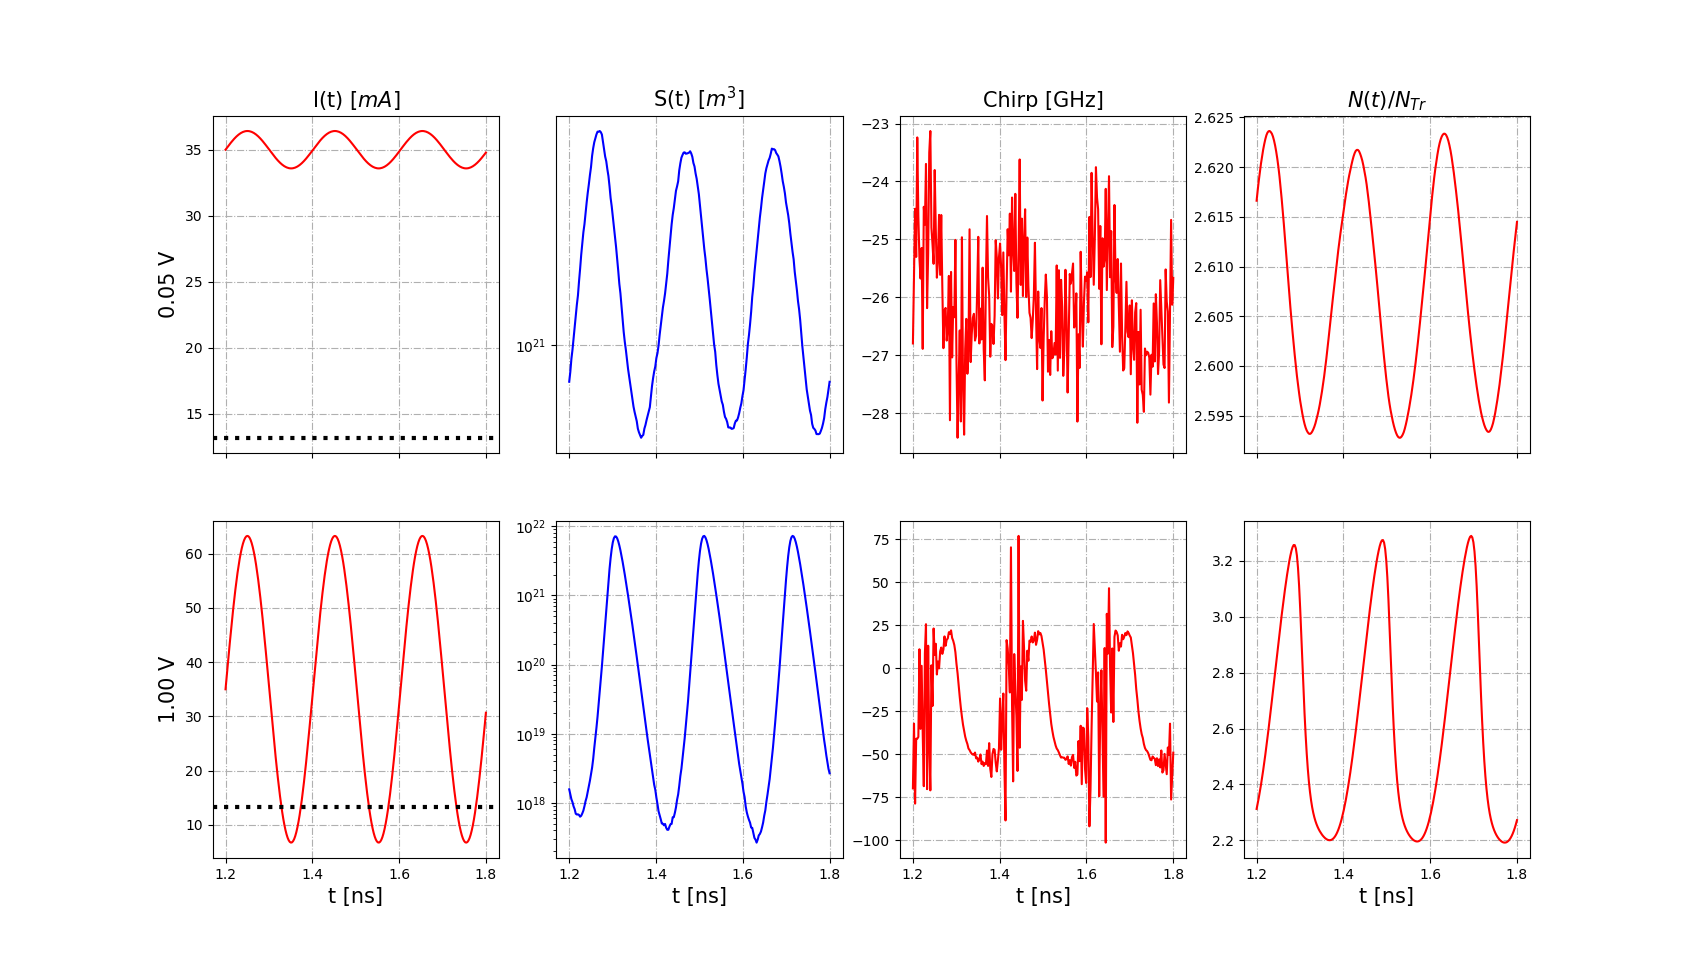
\includegraphics[width=1.0\linewidth]{rateEquations.png}
				\caption{\label{Img:rateEquations}Evolución temporal de la \I ((a)-(c)), la \s ((d)-(f)), la \n\ ((g)-(i)) y del \chirp\ ((j)-(l)) en funci\'on de $V_{RF}$ pasada la zona del transitorio. Para la \I\ se ha marcado la corriente umbral del l\'aser $I_{th} = 14.8$ mA con una l\'inea horizontal discontinua. En la primera columna se muestran las evoluciones temporales para una amplitud de la corriente equivalente a $V_{RF} = 0.05$ V (verde), en la segunda columna para $V_{RF} = 1.00$ V (azul) y en la tercera columna de $V_{RF} = 1.50$ V(naraja).}	
			\end{figure}

		Mientras que para el caso del l\'aser en corriente continua ($I(t) = \ibias$) estudiado en la secci\'on anterior (secci\'on \ref{Sol:CW}), $S(t)$, $N(t)$ y el \chirp\ alcanzaban un valor constante pasado el transitorio, ahora la modulación en la corriente produce oscilaciones de igual periodo en $S(t)$, $N(t)$ y el \chirp. Se observa un aumento de la amplitud en $S(t)$, $N(t)$ y el \chirp\ al aumentar la amplitud de la corriente. Adem\'as, se observa como las oscilaciones en $N(t)$ y el \chirp\ van en fase (m\'aximos en el mismo tiempo $t$), mientras que los m\'aximos de $S(t)$ se obtienen cuando $N(t)$ decae a $N_{th}$.
			
		Para el caso de $V_{RF} = 0.05$ V, con una menor amplitud, se observa que las oscilaciones en la corriente (Figura \ref{Img:rateEquations} (a)) son pequeñas. Al igual que la corriente; la \s, la \n\ y el \chirp\ tambi\'en presentan oscilaciones de amplitud pequeña.% Cabe destacar que para este caso de amplitud pequeña, la \s\ (Figura \ref{Img:rateEquations} (d)) toma valores cercanos a cero, al no producirse ning\'un pico de intensidad. Esto produce que la emisi\'on estimulada no tome valores suficientemente altos como para que la emisi\'on espont\'anea sea despreciable y as\'i, se puede observar en el \chirp\ (Figura \ref{Img:rateEquations} (g)) el ruido debido a la emisión espont\'anea.

		Al aumentar la amplitud de la corriente a $V_{RF} = 1$ V (Figura \ref{Img:rateEquations} (b)) se observa como los aumentos de la corriente durante la oscilaci\'on coinciden con el crecimiento de \n\ (Figura \ref{Img:rateEquations} (k)), haciendo que tome valores muy superiores a $N_{th}$. A su vez, esto produce que, al superar $N(t)$ el valor del umbral $N_{th}$, la \s\ (Figura \ref{Img:rateEquations} (e)) tambi\'en tenga un pico superior al valor del l\'aser en corriente continua. De igual forma que ocurria en el transitorio, al aumentar $S(t)$ y dominar la emisi\'on estimulada, $N(t)$ comienza a disminuir, alcanzando un m\'aximo. Sin embargo, en el momento en el que $N(t)$ alcanza el m\'inimo, la corriente se encuentra por debajo de la corriente umbral $I_{th}$, y $N(t)$ no puede aumentar hasta que $I(t)$ toma nuevamente valores mayores de $I_{th}$. Debido a este tiempo $t$ en el que $N(t)$ no es capaz de volver a aumentar, compensando la disminuci\'on de \s, hay un mayor tiempo $t$ en el que $S(t)$ es cero, y as\'i no hay emisi\'on estimulada. Esta alternancia entre el dominio de la emisi\'on estimulada y la emisi\'on espont\'anea se puede pareciar en el \chirp\ (Figura \ref{Img:rateEquations} (h)), en la que se aprecia el ruido debido a la emisión espont\'anea cuando la densidad de fotones es cero, mienstras que durante los picos de $S(t)$ el ruido es despreciable y no se observa.
			
		Para la amplitud de $V_{RF} = 1.5$ V se observa la misma tendencia que para $V_{RF} = 1$ V, a excepci\'on de que en este caso, al aumentar la amplitud aumenta el tiempo en el que la corriente es menor que $I_{th}$ y as\'i el tiempo en el que $S(t)$ es cero y domina la emisi\'on espontánea.


		En la Figura \ref{Img:PSD} se muestran los espectros de los OFC obtenidos mediante \gs\ para las tres amplitudes de la Figura \ref{Img:rateEquations}.

			% Img:PSD
			\begin{figure}[H]
				\centering
				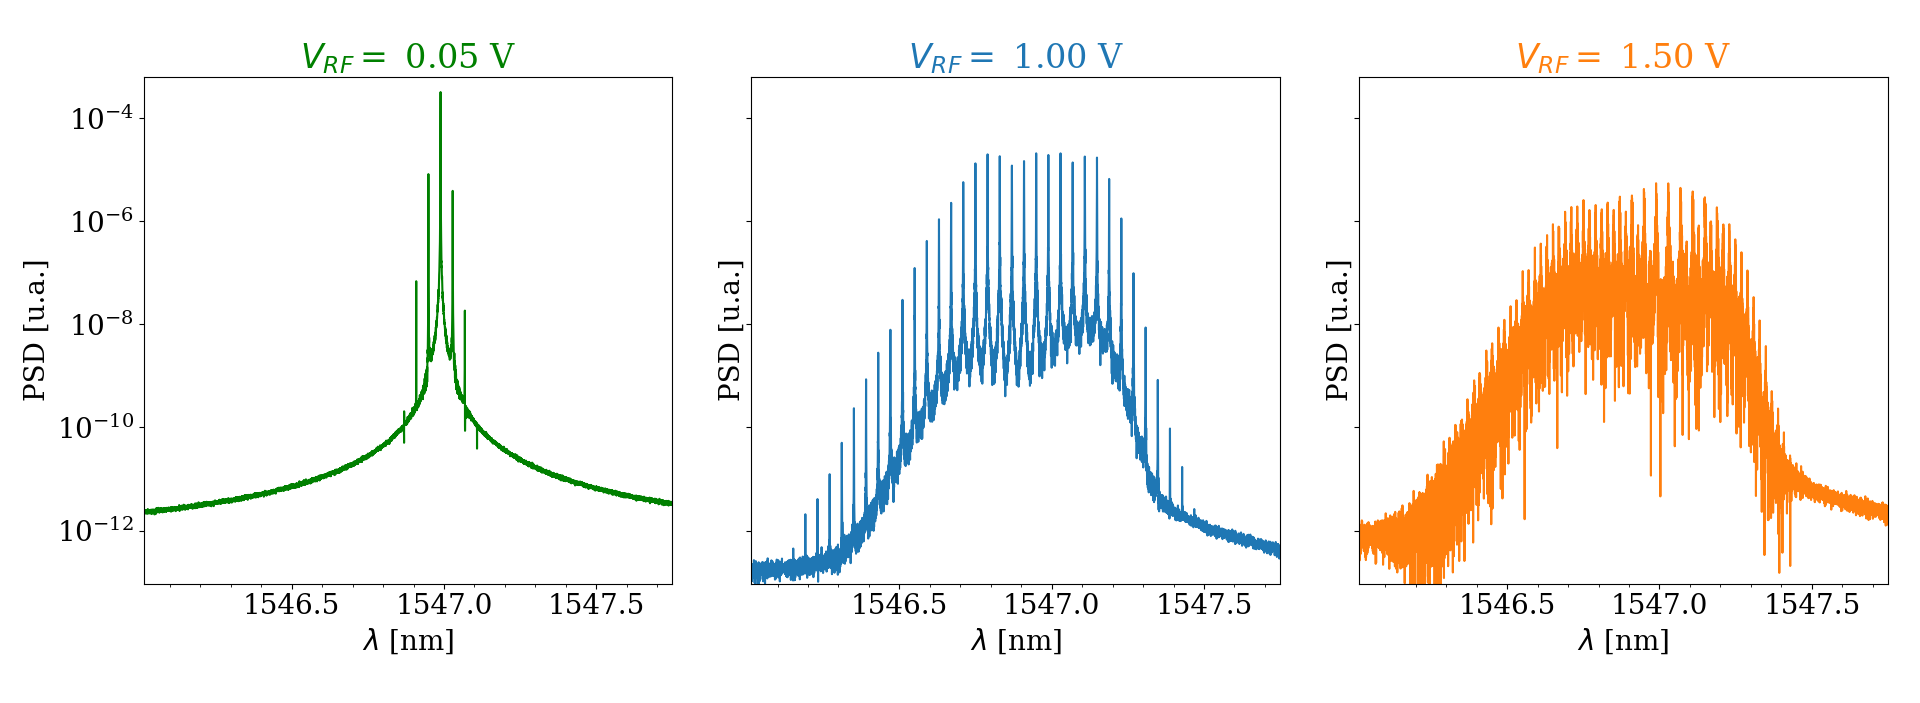
\includegraphics[width=1.0\linewidth]{PSD.png}
				\caption{\label{Img:PSD}Espectros de los OFC obtenidos mediante \gs\ para $\ibias = 30$ mA, $f_R = 5$ GHz y amplitud de modulaci\'on $V_{RF} = 0.05$ V (verde), $1.00$ V (azul) y $1.50$ V (naranja).}
			\end{figure}
			
		Al igual que se obtuvo en la Figura \ref{Img:rateEquations}, se puede observar como el caso de la amplitud de modulaci\'on $V_{RF} = 0.05$ V se asemeja al del l\'aser en corriente cont\'inua, obteniendo un espectro (Figura \ref{Img:PSD} (verde)) con la frecuencia de emisi\'on dominante de la Figura \ref{Img:spectrosCW}. Como consecuencia del \gs\ realizado se observan excitadas las frecuencias de emisi\'on, apareciendo nuebas l\'ineas de emisi\'on a los lados de la emisi\'on principal.

		Para el caso de $V_{RF} = 1$ V se observa un OFC (Figura \ref{Img:PSD} (azul)) de gran calidad formado por numerosas l\'ineas de emisión equiespaciadas y bien definidas. Se ha obtenido una regi\'on de longitudes de onda con l\'ineas de emisión de la misma densidad espectral de potencia lo cuál resulta enuna gran calidad del OFC.

		Por otro lado, se observa que para el caso de $V_{RF} = 1.5$ V (Figura \ref{Img:PSD} (naranja)) el OFC se detruye debido al ruido de la emisión espont\'anea, obteniendo l\'ineas de emisión poco definidas, con un espaciado variado y mucho ruido.

		De esta forma, se ha podido caracterizar la calidad de los OFC, y del \gs, para altas frecuencias en función de la amplitud de modulaci\'on. Se ha podido observar la creaci\'on del OFC para $V_{RF} = 1$ V, as\'i como la destrucci\'on de este para altas amplitudes, con $V_{RF} = 1.5$ V.

		Tal y como se ha comentado a partir de los resultados de la Figura \ref{Img:rateEquations}, uno de los efectos de aumentar la amplitud de modulaci\'on es la disminuci\'on de la corriente por debajo de $I_{th}$ por un tiempo $t$, que aumenta con la amplitud. Sin embargo, \'esto también se puede controlar para una amplitud fija, variando la corriente de polarizaci\'on $\ibias$.

		En la Figura \ref{Img:current} se muestran la potencia $P(t)$, obtenida a partir de la \s\ \ref{eq:Power}, y los espectros de los OFC con $f_R = 5$ GHz, $V_{RF} = 1$ V e $\ibias = 30$ mA y $50$ mA.

			% Img:current
			\begin{figure}[H]
				\centering
				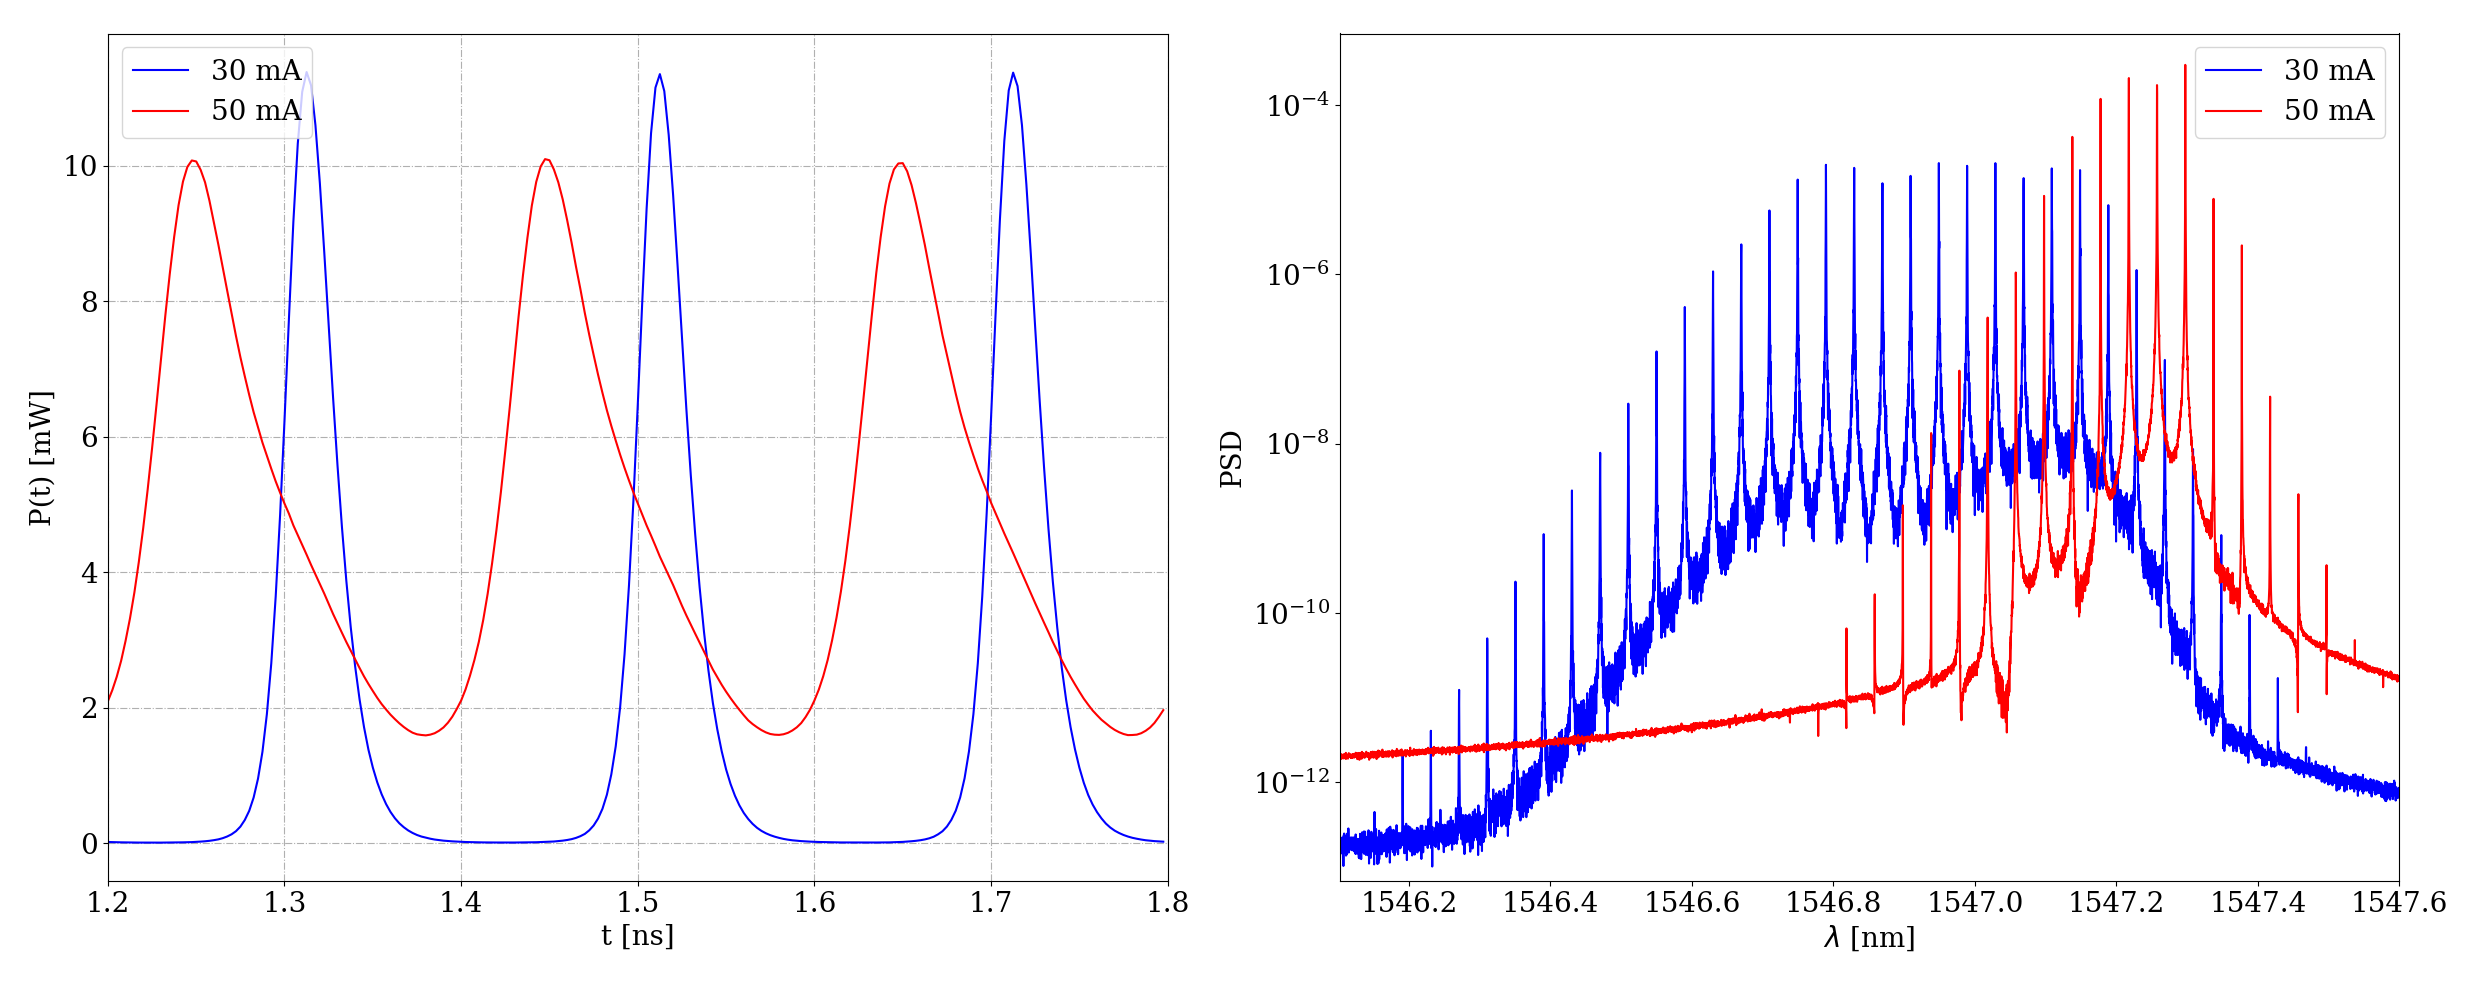
\includegraphics[width=1.0\linewidth]{current.png}
				\caption{\label{Img:current}Perfil temporal de las potencias $P(t)$ (izquierda) y espectros (derecha) de OFC con $f_R = 5$ GHz, $V_{RF} = 1$ V e $\ibias = 30$ mA (azul) y $50$ mA (naranja).}	
			\end{figure}

		En el perfil temporal de la potencia $P(t)$ de $\ibias = 30$ mA (Figura \ref{Img:current} (izquierda, azul)) se observan las zonas de tiempo con $P(t) \propto S(t) = 0$ vistas en la Figura \ref{Img:rateEquations}, debidas a que la corriente toma valores por debajo de $I_{th}$ y as\'i \n\ no puede aumentar. De igual manera se ha obtenido un OFC de gran calidad (Figura \ref{Img:current} (derecha, azul)) como el obtenido en la Figura \ref{Img:PSD}.

		Sin embargo, en el caso de $\ibias = 50$ mA, al aumentar la corriente de polarizaci\'on, \'esta desplaza la función sinusoidal de la intensidad alejandola de $I_{th}$ y as\'i la amplitud de modulaci\'on no es suficiente para llegar a cruzar $I_{th}$. Esto se puede observar en que el perfil temporal de $P(t)$ (Figura \ref{Img:current} (izquierda, naranja)) no toma nunca el valor cero y as\'i realiza oscilaciones completas. Puesto que la frecuencia $f_R$ y la amplitud $V_{RF}$ de modulación s\'i son suficientes com para que se d\'e \gs, se observa un espectro (Figura \ref{Img:current} (derecha, naranja)) con un OFC formado por l\'ineas bien definidas e igualmente espaciadas. No obstante, el OFC obtenido para $\ibias = 50$ mA es m\'as estrecho que el obtenido para $\ibias = 30$ mA, careciendo de una meseta bien definida con l\'ineas de emisi\'on con densidad espectral de potencia similar. Debido a esto, el OFC obtenido para $\ibias = 30$ mA es de mayor calidad que el obtenido para $\ibias = 50$ mA.

		Otro de los efectos de aumentar la $\ibias$ de tal manera que no cruce la $I_{th}$ es la falta de una regi\'on donde domine la emisi\'on espont\'anea, como ocurria en la Figura \ref{Img:rateEquations}. Esto se puede observar en el menor ruido obtenido en el espectro para $\ibias = 50$ mA (Figura \ref{Img:current} (derecha, naranja)) frente al obtenido en el espectro de $\ibias = 30$ mA (Figura \ref{Img:current} (derecha, azul)).

	\addtocontents{toc}{\vspace{0.1cm}}
	\subsection{Efecto de la amplitud de modulación a bajas frecuencias}
		\label{Sol:OFC:LwFreq}

		Para el estudio del efecto de la amplitud de modulación a bajas frecuencias se ha trabajado con una corriente de polarización $\ibias = 50$ mA y una frecuencia $f_R = 500$ MHz. Se han obtenido la potencia $P(t)$ y los OFC para cuatro amplitudes diferentes, tomando cuatro valores distintos para $V_{RF}$: $0.05$ V, $0.4$ V, $1.0$ V y $1.2$ V.

		En la Figura \ref{Img:500} se muestran los perfiles temporales de la potencia $P(t)$ y los espectros de los OFC para $\ibias = 50$ mA, $f_R = 500$ MHz y $V_{RF} = 0.05$ V, $0.4$ V, $1.0$ V y $1.2$ V.
			% Img:500
			\begin{figure}[H]
				\centering
				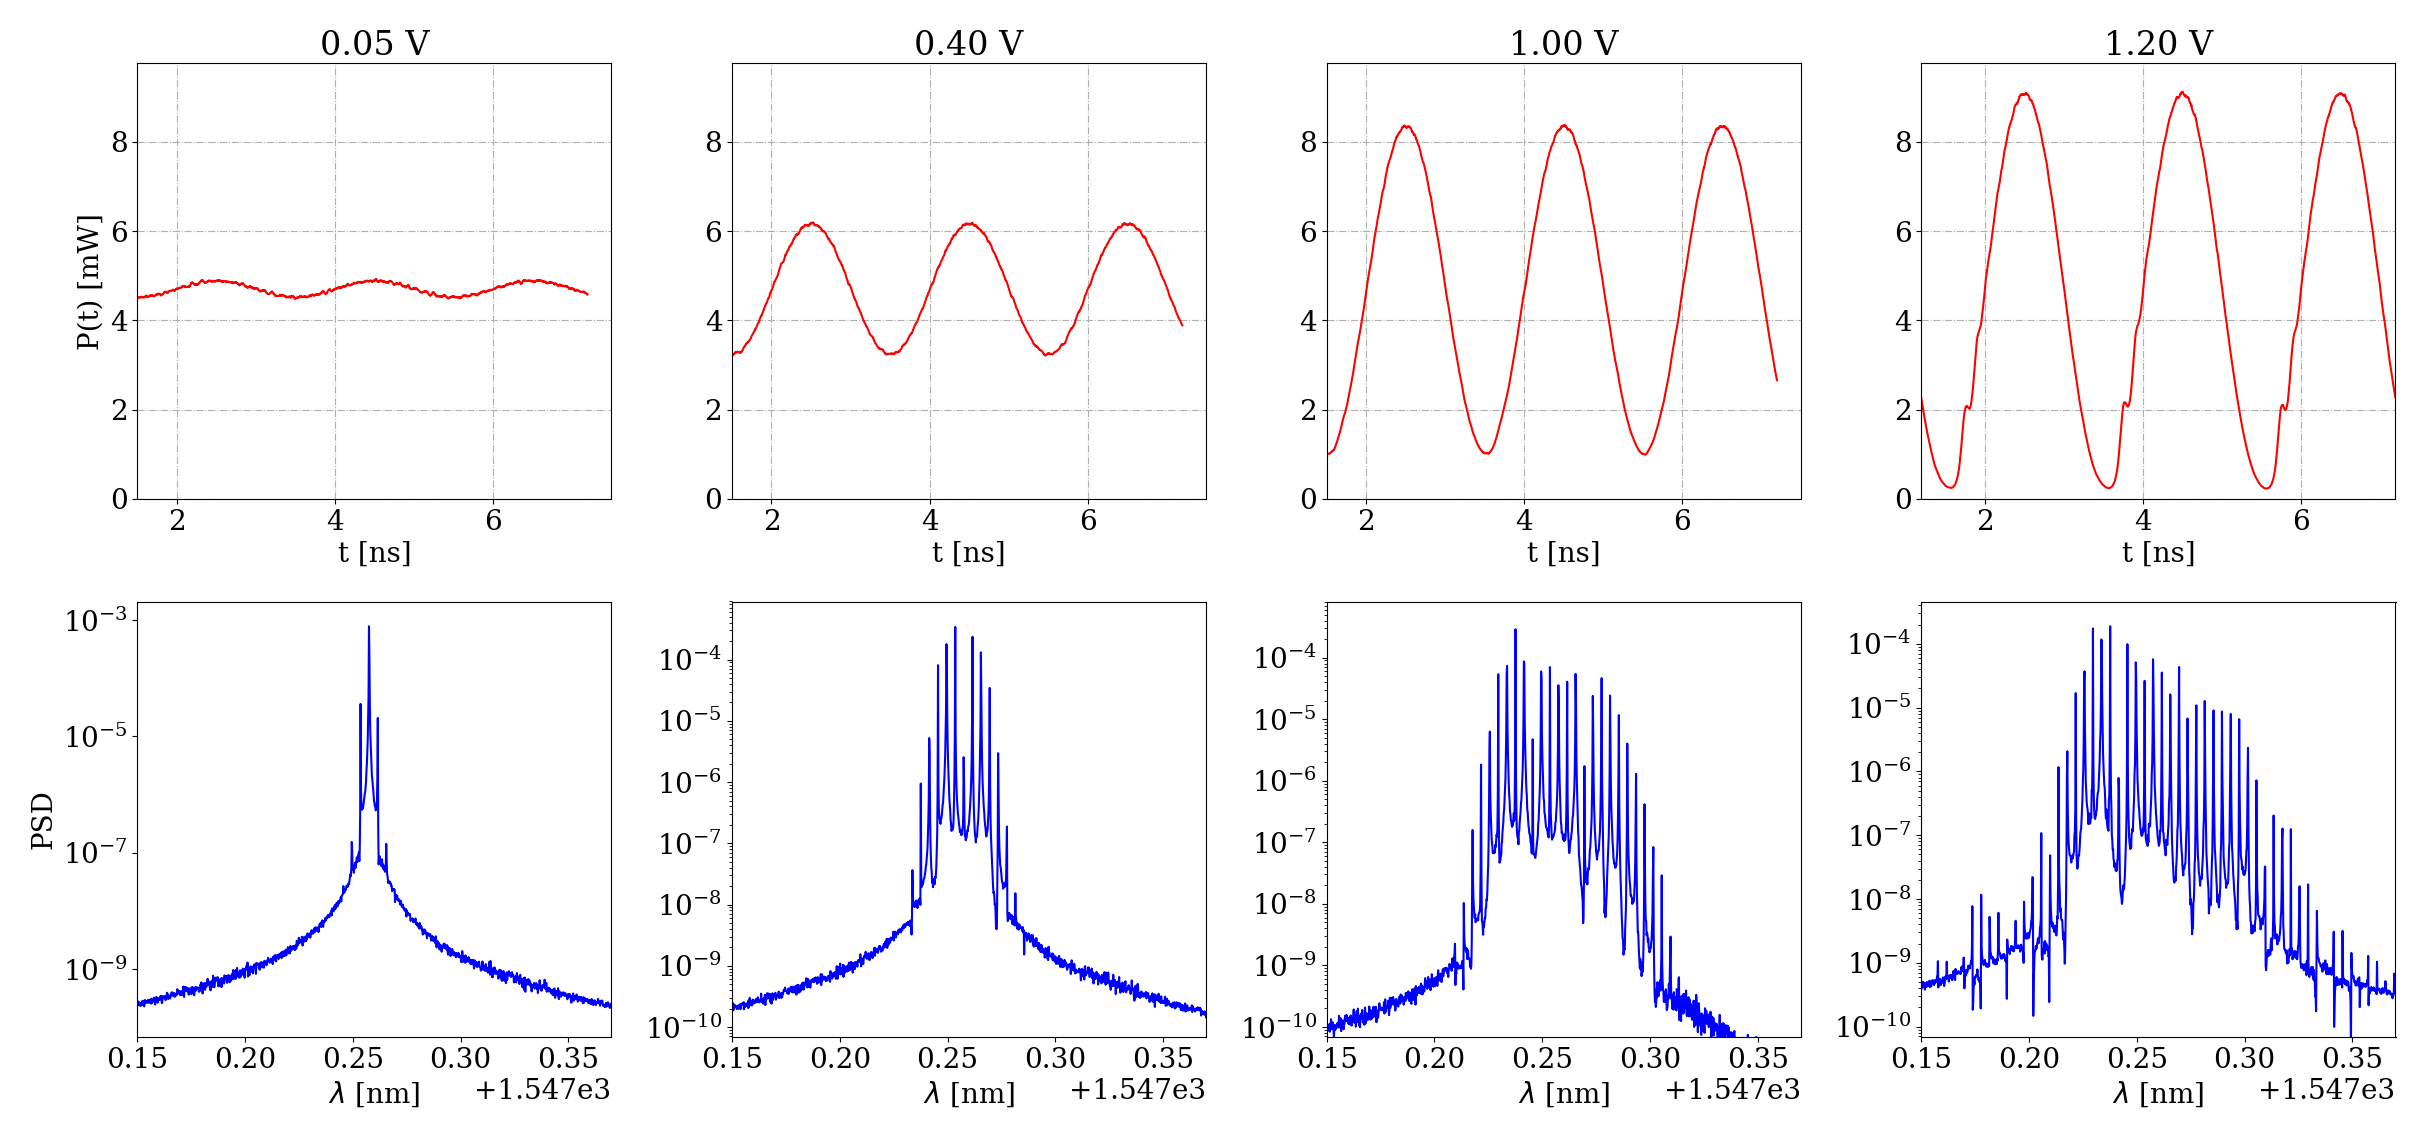
\includegraphics[width=1.0\linewidth]{500.png}
				\caption{\label{Img:500}Perfiles temporales de la potencia $P(t)$ (fila superior) y espectros (fila inferior) de los OFC para $\ibias = 50$ mA, $f_R = 500$ MHz y $V_{RF} = 0.05$ V (primera columna), $0.4$ V (segunda columna), $1.0$ V (tercera columna) y $1.2$ V (cuarta columna).}	
			\end{figure}

		Al igual que se obtuvo en el apartado anterior para el caso de altas frecuencias con $\ibias = 50$ mA (Figura \ref{Img:current}), se observan en la Figura \ref{Img:500} perfiles temporales de la potencia oscilantes entorno al valor de la potencia en corriente continua ($P_{CW} \approx 4.7$ mW), variando su amplitud en funci\'on de la amplitud de modulación. Al tener una $\ibias$ muy superior a $I_{th}$ y una frecuencia baja, la amplitud de modulaci\'on no permite mantener la corriente de inyecci\'on por debajo de la corriente umbral un tiempo suficiente como para que $P(t) \propto S(t) = 0$, tal y como se observa en las Figuras \ref{Img:500} (fila superior).

		Para el caso de la amplitud de modulaci\'on pequeña con $V_{RF} = 0.05$ V, se ha obtenido un comportamiento muy similar a la corriente continua, al igual que para altas frecuencias. El espectro obtenido para esta amplitud de modulaci\'on es similar al de la Figura \ref{Img:PSD} (verde) del apartado anterior, obteniendo un pico de emisi\'on dominante correpondiente a la emisi\'on en continua y dos picos a cada lado debidos a la excitaci\'on de la frecuencia de oscilación.

		Se observa como, al igual que ocurria en a altas frecuencias, a medida que aumenta la amplitud de modulación aumenta el n\'umero de l\'ineas de emisión de espectro, llegando a destruirse para altas amplitudes de modulación. Sin embargo, al trabajar a bajar frecuencias se observa una clara irregularidad en el perfil del OFC, tomando los picos valores muy diversos de la densidad espectral de potencia. Esto implica una perdida de la calidad de los OFC a bajas frecuencias con respecto a altas frecuencias. 

		DEBERIA HABLAR SOBRE LOS PICOS QUE SE OBSERVAN EN LA POTENCIA PARA V = 1.2

		En la Figura \ref{Img:500mhz} se muestran los perfiles temporales de la potencia $P(t)$ y los espectros de los OFC para $\ibias = 50$ mA, $f_R = 500$ MHz y $V_{RF} = 0.1$ V, $0.4$ V, $1.2$ V y $1.6$ V obtenidos experimentalmente \cite{Chaves19}.

			% Img:500mhz
			\begin{figure}[H]
				\centering
				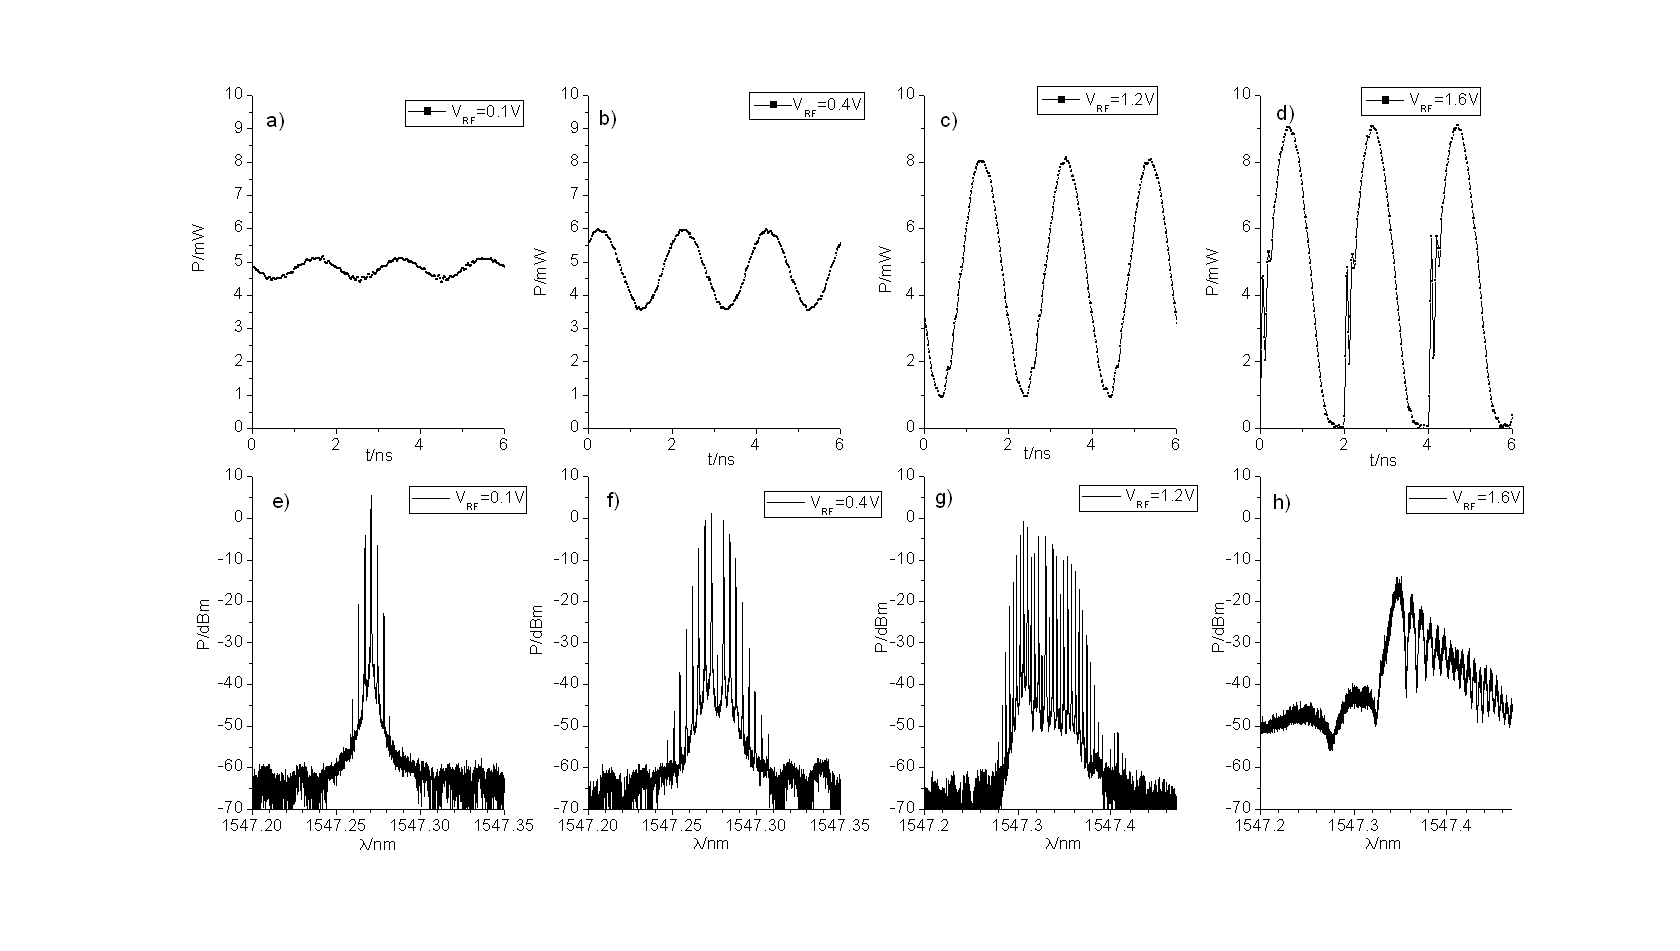
\includegraphics[width=1.0\linewidth]{../Chaves/OFC-GS/500mhz.png}
				\caption{\label{Img:500mhz}Perfiles temporales de la potencia $P(t)$ (fila superior) y espectros (fila inferior) de los OFC para $\ibias = 50$ mA, $f_R = 500$ MHz y $V_{RF} = 0.1$ V (primera columna), $0.4$ V (segunda columna), $1.2$ V (tercera columna) y $1.6$ V (cuarta columna) obtenidos experimentalmente \cite{Chaves19}.}	
			\end{figure}

		En la Figura \ref{Img:500mhz} se muestran la potencia $P(t)$ y los espectros experimentales para diferentes amplitudes de modulación, permitiendo comparar los resultados obtenidos mediante simulación con los obtenidos en el laboratorio.

		En la cuarta columna de la Figura \ref{Img:500mhz} se muestran los resultados obtenidos para una amplitud de $V_{RF} = 1.6$ V, observando como el espectro de frecuencia se encuentra completamente destruido. Dichos resultados no pudieron ser obtenidos mediante la simulación debido al problema en el transitorio con $\sqrt{S(t)}$. En la primera columna de la Figura \ref{Img:500mhz} se muestran los resultados para una amplitud de modulación pequeña de $V_{RF} = 0.1$ V. Al igual que en los resultados de la simulación, se obtiene un comportamiento similar al de la corriente continua con un pico de emisi\'on dominante. No obstante, al tratarse de el doble de la amplitud utilizada en la simulaci\'on de la Figura \ref{Img:500} se obtienen un mayor n\'umero de picos de emisión estimulados. Los resultados que se muestran en la segunda columna de la Figura \ref{Img:500mhz}  para $V_{RF} = 0.4$ V equivalen a los resultados de la simulación de la segunda columna de la Figura \ref{Img:500}. En ambas figuras se pueden observar un OFC con un perfil aproximandamente sim\'etico con un pico de menor intensidad en el centro. Por \'ultimo, la tercera columna de la Figura \ref{Img:500mhz} equivale a la cuarta columna de la Figura \ref{Img:500}. Ambos espectros presentan un perfil similar con un aumento brusco de la densidad espectral de potencia de los picos para bajas longitudes de onda, seguido de una disminuci\'on m\'as tenue para lontitudes de onda mayores. Ambos perfiles temporales de potencia presentan LOS PICOS DE LOS QUE HE DE HABLAR.

	El excelente acuerdo entre los resultados de la simulaci\'on de la Figura \ref{Img:500} y los resultados experimentales de la Figura \ref{Img:500mhz} indican la capacidad de la simulaci\'on de explicar los procesos que involucra el \gs\ en la generaci\'on de OFC, pudiendo servir para la caracterizaci\'on de la calidad de los OFC.
